\documentclass[a4paper, top=10mm]{article}
%for writing from the top
\usepackage{fullpage}
%for math
\usepackage{amsmath}
\usepackage{mathrsfs}
\usepackage{amsthm}
%for images
\usepackage{graphicx}
%for color
\usepackage{xcolor}
%for title
\title{\textbf{\huge{New Santa's Sleigh}}}
\author{Enigma n\textsuperscript{o}7}
\date{14\textsuperscript{th} December 2023}

\newtheorem*{hint}{Hint}

\addtolength{\voffset}{-2cm}
\addtolength{\textheight}{5cm}


\begin{document}
	\maketitle
	
	Santa's magical reindeer are getting old.
	In order to have no disruption in the distribution of presents when the reindeer can no longer fly, Santa is testing a new model of sleigh from the future: a laser-powered sleigh.
	
	The concept is simple: Santa Clause needs to ask the elves to construct towers at regular intervals.
	They will take it in turns to propel the sleigh via ultra-powerful lasers.
	To prevent the sled from disintegrating, it is fitted with a shield at the rear.
	
	\begin{center}
		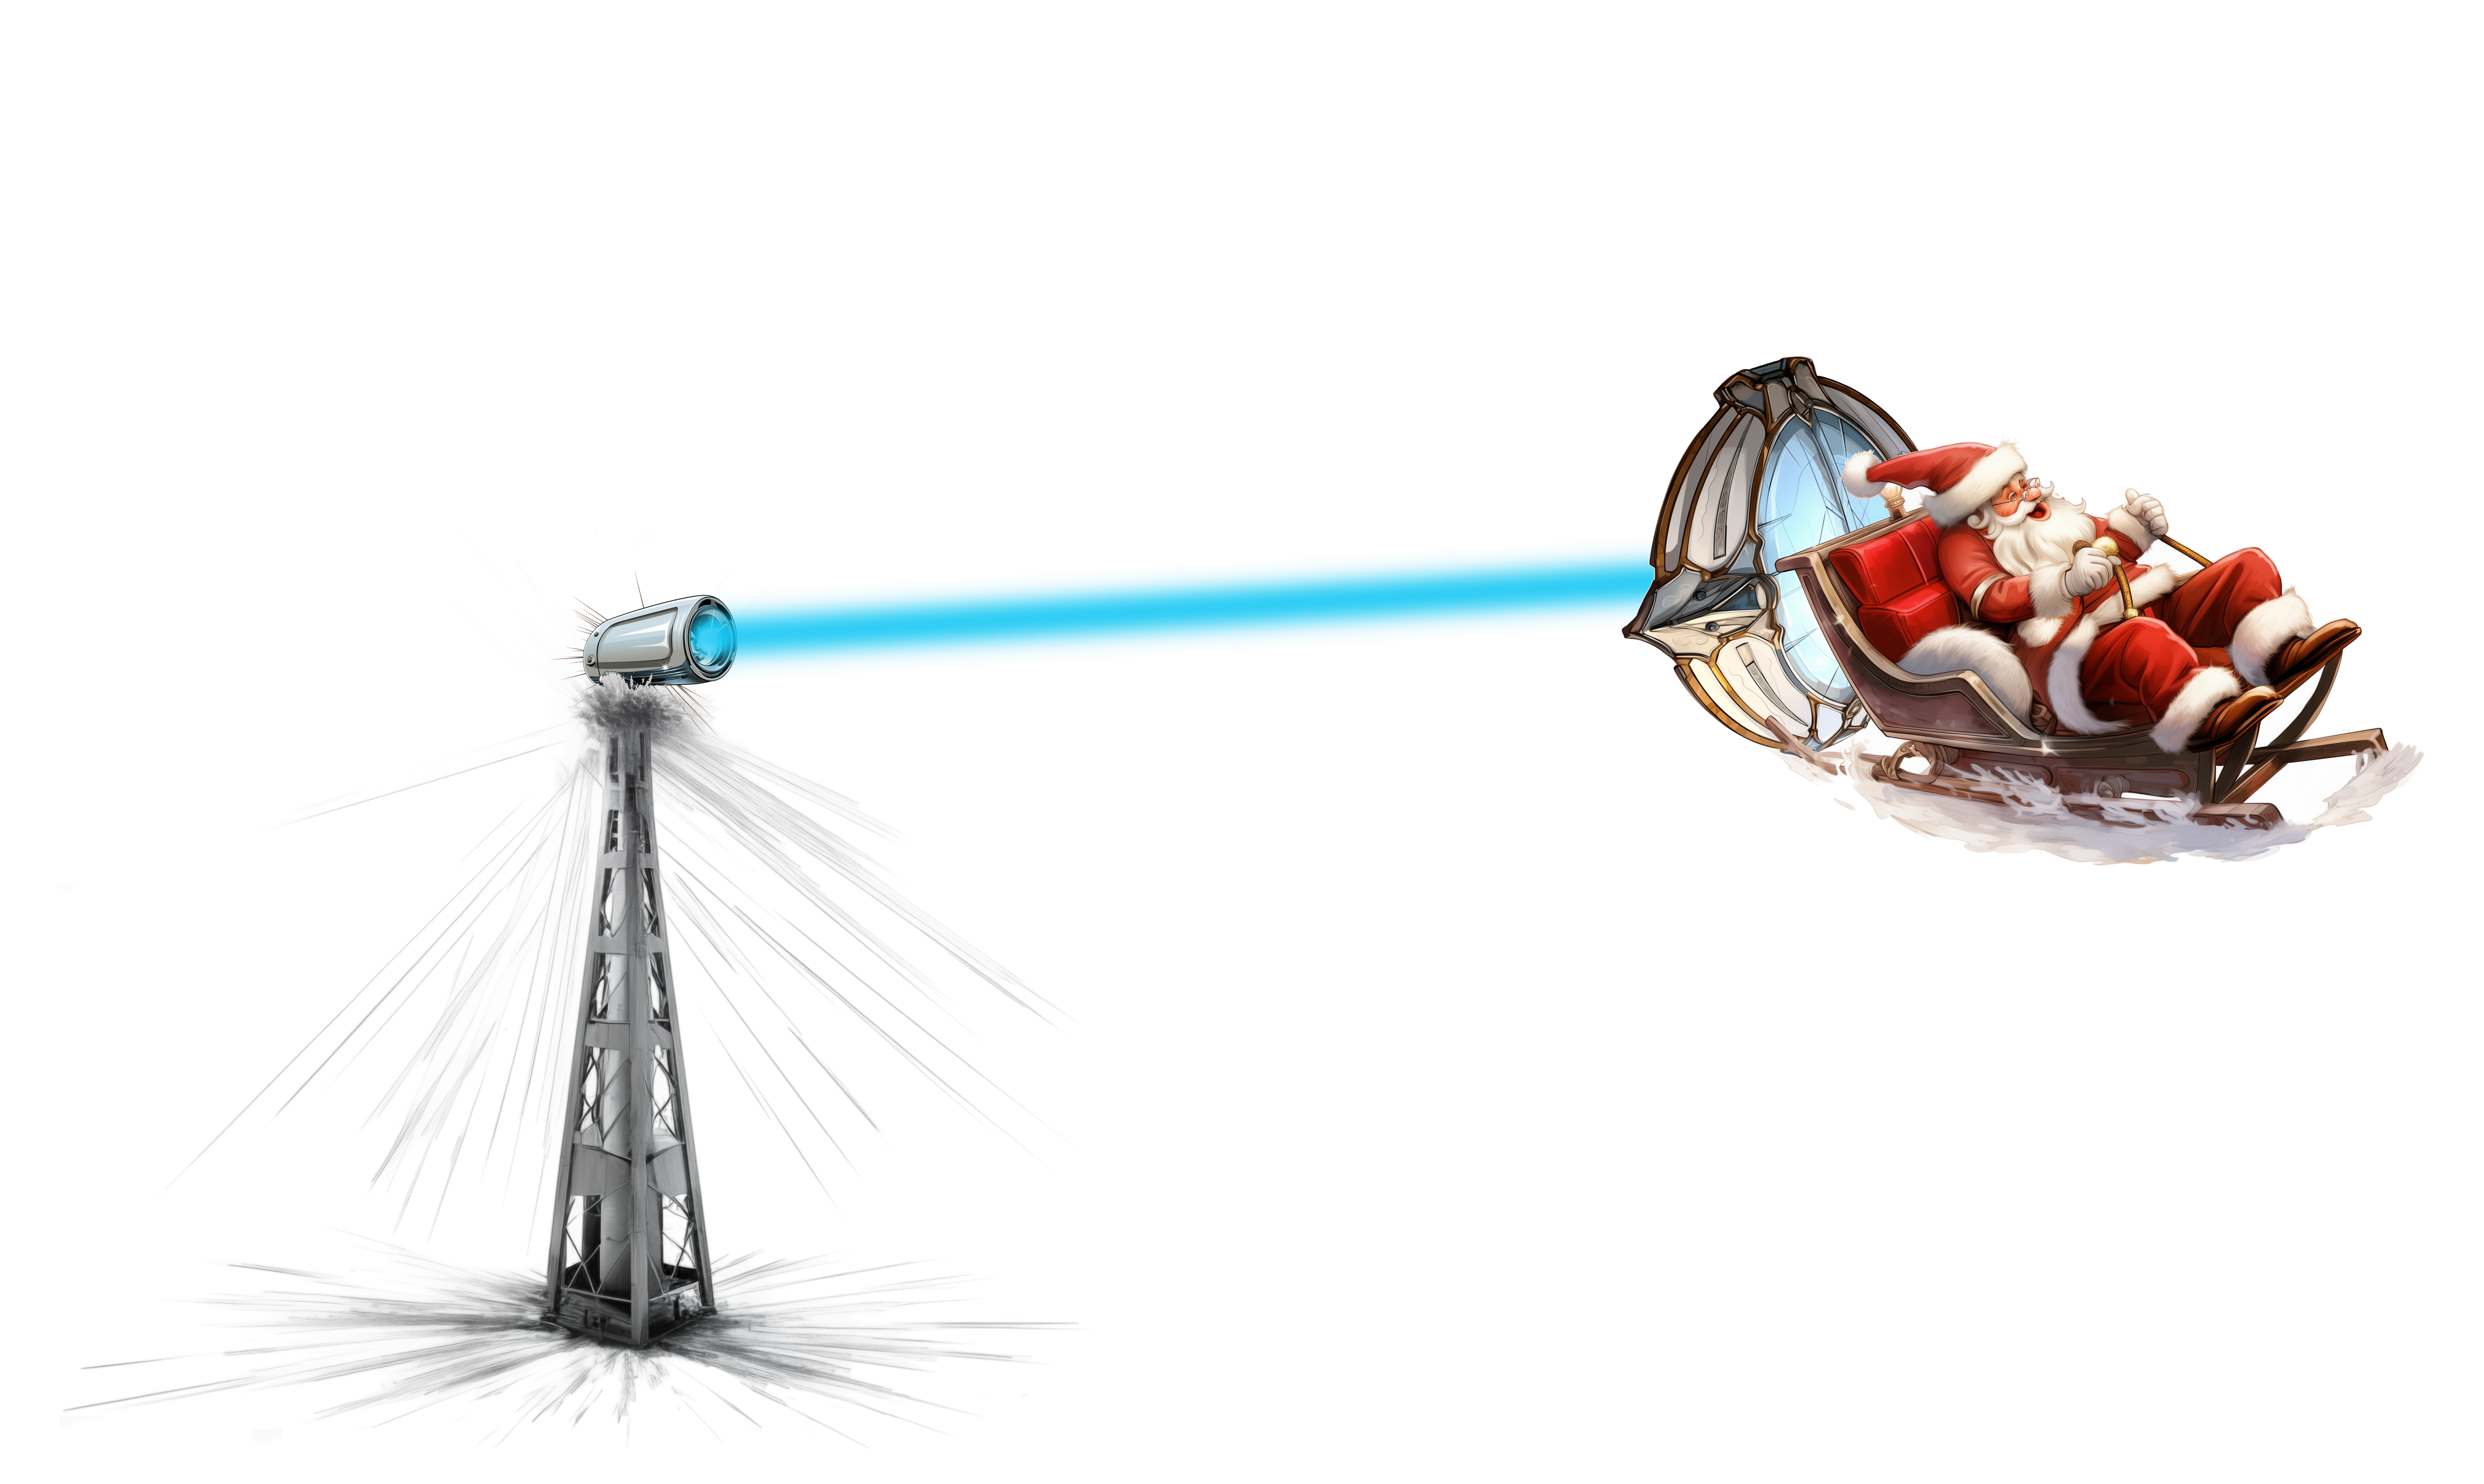
\includegraphics[width=\linewidth]{07full.png}\\
		Santa Clause trying his new high-tech sleigh.
	\end{center}
	
	If $D$ id the distance between the sleigh and the tower, the energy transmitted by the tower is proportional to $1/D$ (due to interaction of the laser with the atmosphere).
	The velocity $V$ of the sleigh is proportional to the energy it receives from the tower (1).
	Despite the shield, being to close to the tower is dangerous (2).
	The sleigh is launched via a big spring canon, configured so that the sleigh arrives at flying altitude at the beginning of the safe range of the first tower (3).
	There is a minimum speed, below that speed, the sleigh cannot fly properly (4).
	
	\begin{enumerate}
		\item We have $V = \frac{\beta}{D}$\footnote{With $V$ in m/s and $D$ in m (meters).}, with $\beta=4\,000\,000$s$ ^{-1}$.
		\item The sleigh must be at least $8$km away from the tower (when receiving energy from the tower)
		\item The canon is configured so that the sleigh arrives with a speed of $900$km/h ($250$m/s) at $8$km from the first tower (at $t=0$s).
		\item The sleigh can not fly at a speed below $144$km/h ($40$m/s).
	\end{enumerate}
	
	\textbf{What is the maximal possible distance (in meters) between two towers?}
	
\end{document}